\chapter{РАЗРАБОТКА МОДУЛЕЙ}
% \chapter{Разработка модулей}

\section{Выбор стека технологий}

\subsection{Группы используемых технологий}
Перед началом реализации разработанной архитектуры необходимо выбрать
стек технологий, которые будут использоваться при разработке.
Необходимо определиться со следующими пунктами:
\begin{itemize}
    \item операционная система
    \item гипервизоры
    \item реализация управляющей логики
\end{itemize}
Касательно гипервизоров, необходимо выбрать способ виртуализации обычных виртуальных машин
и сетевого оборудования.

\subsection{Операционная система}
В качестве операционной системы предпочтительнее всего использовать Linux, так как ее 
администрирование не представляет собой большой проблемы, она бесплатна и имеет
открытый исходный код и отличную поддержку большинства современных языков 
программирования. Кроме этого, для администрирования Linux существуют доказавшие
свою эффективность системы автоматизации установки и администрирования, \cite{chef} \cite{puppet} \cite{fabric} что совершенно
необходимо для успешной поддержки многомашинных систем.

\subsection{Гипервизоры}
Если говорить о виртуализации сетевого оборудования, то имеется два пути: использовать
специализированные гипервизоры, или же использовать стандартные гипервизоры вместе с
программными коммутаторами, такими как Open vSwitch. На текущий момент, программные
коммутаторы редко используются при создании сетей в предприятиях, поэтому большого
смысла поддерживать этот вариант нет. По данным Infonetics Research, Cisco занимает
лидирующие позиции на рынке сетевого оборудования, \cite{infonetics-cisco}
поэтому выбор этого сетевого оборудования в качестве цели для виртуализации вполне оправдан.
Кроме этого, гипервизор dynamips, предназначенный для эмуляции именно этого оборудования,
является самым распространенным и стабильным в своей области. %TODO источник

Среди гипервизоров PC-совместмого оборудования можно выделить несколько наиболее
популярных решений для Linux:
\begin{itemize}
    \item VmWare ESX
    \item VirtualBox
    \item Xen
    \item KVM
\end{itemize}

VmWare ESX является одним из наиболее популярных коммерческих гипервизоров, но при 
использовании в рамках данного проекта имеет ряд недостатков. Во-первых, гипервизор
работает только со специальным образом модифицированным ядром ОС, во-вторых,
данный гипервизор имеет закрытый код, и в случае необходимости становится невозможным
внести изменения, необходимые для реализации проекта.

VirtualBox -- гипервизор с открытым исходным кодом, в данный момент поддерживаемый 
компанией Oracle. Данный продукт в основном базируется как решение для настольных
компьютеров, несмотря на возможность работы без графического интерфейса.
Ранее VirtualBox разрабатывался компанией Sun, которая была куплена Oracle в 2010 году.
Переход многих программ с открытым исходным кодом во владение к Oracle сказался на
их поддержке крайне негативно, поэтому в долгосрочной перспективе использование
VirtualBox при реализации данного проекта не имеет большого смысла при наличии альтернатив.

Xen долгое время был выбором по-умолчанию в Linux-среде и активно поддерживался
самой большой Linux-компанией -- RedHat. %TODO источник
Тем не менее, последние несколько лет интерес к нему падает, так как
RedHat переключил свой фокус на KVM. Так же, в силу того, что этот гипервизор 
использует технику паравиртуализации, его администрирование имеет ряд отличий
от администрирования обычных Linux-систем.

KVM -- относительно новый, но уже достаточно популярный и стабильный Linux-специфичный
гипервизор. На данный момент он активно поддерживается, в том числе коммерческими компаниями,
такими как RedHat, и на настоящий момент является выбором по-умолчанию для виртуализации в 
Linux. Кроме этого, благодаря открытому коду, в него будет возможно внести изменения,
если такая необходимость возникнет во время разработки.
Таким образом, в качестве гипервизора PC-совместимых виртуальных машин в данном проекте
будет использоваться KVM.

\subsection{Способ описания управляющей логики}
При разработка управляющей логики имеется два варианта: писать весь необходимый код с нуля, 
используя только стандартные библиотеки языков, или же расширить возможности имеющейся
платформы. Написание кода с нуля с одной стороны позволяет получить полный контроль 
над кодовой базой и выбором технологий, но с другой стороны -- потребует реализации
большого объема относительно стандартной логики, которая не имеет большого отношения 
к сути данной работы. Гораздо более оптимальным вариантом является использование уже 
существующих наработок.

Как нельзя кстати в данном случае подходит платформа OpenStack. Рассматривая компоненты,
из которых она состоит, можно отметить, что архитектура этой платформы хорошо вписывается
в модель реализации, разработанную в предыдущей главе.
Большинство компонент OpenStack может быть использовано в 
системе моделирования сетей либо напрямую, без всякой модификации, либо путем
написания соответствующего расширяющего кода. Список компонентов, подлежащих
повторному использованию, представлен в табл.~\ref{tab:openstack-reuse}
\begin{table}
\center
\caption{Возможность повторного использования компонент OpenStack}
\label{tab:openstack-reuse}
\begin{tabular}{|p{5cm}|p{4cm}|p{5cm}|} \hline 
\multicolumn{3}{|c|}{обработка запросов} \\ \hline 
авторизация и аутентификация & keystone & без изменений\\ \hline
логика команд & - & необходима реализация \\ \hline
\multicolumn{3}{|c|}{хранение данных} \\ \hline
получение образов ОС & glance & без изменений \\ \hline
хранение виртуальных дисков & на узлах nova-compute или в nova-volume & без изменений\\ \hline
\multicolumn{3}{|c|}{управление виртуальными машинами} \\ \hline
планировка ресурсов & nova-scheduler & без изменений \\ \hline
настройка сети & quantum & необходим дополнительный модуль \\ \hline
управление гипервизором & nova-compute & необходим дополнительный модуль \\ \hline
\hline 
\end{tabular} 
\end{table}

Путем использования уже существующей платформы, при реализации системы моделирования
сетей мы избегаем реализации большого количества не относящейся к сути логики. В итоге мы
получаем три группы модулей, требующих реализации:
\begin{enumerate}
    \item высокоуровневый прикладной программный интерфейс
    \item сетевое взаимодействие
    \item запуск специфических виртуальных машин -- маршрутизаторов в гипервизоре dynamips
\end{enumerate}

Прикладной программный интерфейс должен работать в терминах разработанной модели данных.
Следуя концепции модульной архитектуры, он будет реализован в виде отдельного процесса,
и будет транслировать высокоуровневые вызовы пользователя в ряд вызовов к нижележащим
подсистемам: nova-api и quantum.

Модель сети, которая используется внутри OpenStack по-умолчанию устроена так, что 
все виртуальные машины одного проекта находятся в одной подсети. Тем не менее,
используя последние наработки сообщества разработчиков этой платформы, возможно использование
quantum для гибкой настройки соединения между виртуальными машинами.

Для того, чтобы конфигурировать сеть между виртуальными машинами в OpenStack на 
канальном уровне, необходимо реализовать два аспекта. Во-первых, необходим такой способ 
инкапсуляции кадров канального уровня, который позволит запускать достаточно большое
количество виртуальных машин в одной системе, обеспечивая изоляцию между ними.
Во вторых, необходимо предоставлять данные о физических портах в подсистему виртуализации.

Проекты GNS3 и dynagen решают проблему инкапсуляции при помощи использования UDP-каналов.
Для работы dynamips совместно с KVM при данном подходе ранее было необходимо использование 
специально модифицированной версии Qemu, но на настоящий момент UDP-каналы
поддерживаются и в официальной версии эмулятора.

Проблема предоставления данных о физических портах в систему виртуализации вытекает
из ограниченной сетевой модели OpenStack, которая использовалась с самого начала разработки
проекта. Вместо явного указания количества виртуальных сетевых адаптеров и способа их 
соединения с сетями, в nova-compute передавался только список сетей, к которым необходимо
подключить виртуальную машину. По этой причине не существует стандартного способа передачи
таких метаданных о подключенной сети, как номер сетевой карты и порта.
Для решения проблемы метаданных портов в рамках этого проекта создано расширение прикладного 
программного интерфейса Quantum, позволяющее задавать и получать метаданные порта.

Архитектура nova-compute изначально была расчитана на поддержку различных гипервизоров.
Благодаря этому, для поддержки виртуализации сетевого оборудования системой моделирования
сетей, необходимо создать так называемый драйвер гипервизора. Интерфейс драйвера гипервизора
содержит около 60 методов, из которых далеко не все обязательны для реализации, и
в нашем случае задача сводится к созданию обертки над dynagen, которая конфигурирует
виртуальные маршрутизаторы согласно информации, полученной от прикладного программного
интерфейса и расширения Quantum для метаданных.

\section{Описание прикладного программного интерфейса}
\subsection{Базовый протокол}

Интерфейс программирования приложений (иногда интерфейс прикладного программирования) (англ. application programming interface, API) --  набор готовых классов, процедур, функций, структур и констант, предоставляемых приложением (библиотекой, сервисом) для использования во внешних программных продуктах.

API определяет функциональность, которую предоставляет программа (модуль, библиотека), при этом абстрагируя конкретную реализацию этой функциональности. Благодаря API возможно создание
программ, взаимодействующих с другими программами.

Так как в рамках данной работы делается акцент на разработку логики системы моделирования сетей,
разработанная реализация не имеет графического пользовательского интерфейса. Вместо этого,
система предоставляет свой собственный API для взаимодействия, оперирующий в терминах 
модели предметной области.

На настоящий момент, наиболее часто используемым способом организации взаимодействия
программ по сети является REST. REST (Representational State Transfer, «передача представлений 
состояний») не имеет в основе конкретного стандарта, и является не более чем стилем построения 
архитектуры распределенного приложения. Принципы REST были впервые описаны в диссертации
одного из разработчиков протокола HTTP, Роя Филдинга.\cite{restapi}

Как правило, под REST сервисами подразумеваются сервисы, которые предоставляют пользователю
доступ к некоторому набору ресурсов, с которыми можно взаимодействовать посредством
HTTP-запросов. При этом ресурсы кодируются в одном или нескольких возможных заранее
определенных форматах, как правило человекочитаемых, таких как XML или JSON.
В данном случае в качестве формата используется JSON, так как он является более компактным
и легкочитаемым по сравнению с XML, а так же наиболее распространенным на данный момент.

Несмотря на то, что сам по себе REST не является стандартом, существуют стандарты на описание
интерфейсов REST-сервисов. Если для представления данных используется JSON, то можно
применить стандарты JSON Schema и JSON Hyper-Schema. Первый стандарт позволяет
регламентировать формат представления ресурсов: имена полей, типы данных и т.д. Второй
стандарт расширяет JSON Schema, позволяя задавать ссылки на связанные ресурсы, а так же
ссылки на действия над данным ресурсом.

OpenStack использует для аутентификации сервис Keystone. Перед работой с системой, пользователь
должен сначала получить так называемый токен у Keystone, который необходимо отправлять в 
заголовке HTTP-запроса \verb`HTTP_X_AUTH_TOKEN` при обращении к Nova, Glance и другим сервисам. 
В целях унификации, прикладной программный интерфейс системы моделирования так же будет 
использовать Keystone для своей работы.

Как и в OpenStack, пользователи системы сгруппированы в группы, называемые тенантами 
(англ. tenants). Так как с одной стороны, разные группы пользователей в перспективе могут иметь 
разные картотеки сущностей, а с другой стороны REST подразумевает, что содержимое 
ресурса полностью описывается его URL, то принято решение ко всем адресам сущностей добавить
в виде префикса идентификатор группы.

При выделении сущностей в ресурсы необходимо поддерживать баланс между гранулярностью
и денормализованностью. Слишком большая гранулярность делает описание API раздутым и сложным,
а слишком денормализованное -- увеличивает количество передаваемых данных, и зачастую 
требует большого количества кода для извлечения желаемых сущностей из представления ресурса.

Анализируя предполагаемую работу с системой, можно выделить следующие наиболее частые действия:
\begin{itemize}
   \item создание, получение и удаление топологии
   \item получение списка типов узлов для запуска новой топологии со стандартным 
            набором сетевых адаптеров для узла
   \item получение списка типов сетевых адаптеров для запуска новой топологии, в которой
            к узлам подключены сетевые адаптеры, отличные от конфигурации по-умолчанию
\end{itemize}

Таким образом, можно выделить три ресурса:
\begin{itemize}
    \item типы узлов
    \item типы сетевых адаптеров
    \item топологии
\end{itemize}
Первые два должны изменяться только административно, последние же -- самим пользователем.

\subsection{Типы сетевых адаптеров}

%TODO реализовать параметры в коде
Тип сетевого адаптера имеет три атрибута: имя $name$ и список портов $ports$. 
Доступные типы сетевых адаптеров представлены
в виде единого ресурса, благодаря чему при редактировании топологии можно единожды
запросить список адаптеров и использовать его в дальнейшем.  Для упрощения кода на стороне 
пользователя, множество доступных адаптеров задается в виде объекта JSON с ключами,
равными имени типа адаптера. URL для ресурса будет иметь вид \verb`/{tenantid}/cards`, ресурс не изменяем
для пользователей. 

JSON-схема ресурса, таким образом, принимает следующий вид:

\lstinputlisting{schema/schema_slots.json}

Что соответствует подобному JSON-документу:

\lstinputlisting{code/slots.json}


\subsection{Типы узлов}

Типы узлов имеют следующие аттрибуты: идентификатор $id$, человекочитаемое название
$name$, список портов для подключения сетевых адаптеров $slots$, 
набор параметров $parameters$, список доступных для запуска версий операционных систем 
$software$, а так же набор метаданных $metadata$. Сетевые адаптеры
по-умолчанию указаны напрямую в списке портов.
Так же, как и типы сетевых адаптеров, типы представлены в виде единого ресурса, объединенные в 
объект JSON. URL ресурса -- \verb`/{tenantid}/devices`, для пользователя этот ресурс доступен только 
для чтения.

JSON-схема типов узлов имеет следующий вид:

\lstinputlisting{schema/schema_hardware.json}

Что соответствует следующему JSON-документу:

\lstinputlisting{code/hardware.json}


\subsection{Топологии}

Топологию, как было рассмотрено ранее, можно разделить на список узлов и список 
связей. При этом каждый узел имеет идентификатор $id$, человекочитаемое название
$name$, список слотов с подключенными адаптерами $slots$, 
набор значений параметров $parameters$, версию операционной системы $software$, 
а так же набор метаданных $metadata$. 

В целях упрощения реализации будем считать, что каждая связь может иметь только два 
подключенных порта  $left$ и $right$, и не имеет каких-либо специфических параметров.
Так же, каждое соединение имеет идентификатор связи $id$.

Топологии являются единственными ресурсами, которые может редактировать пользователь.
Они доступны по URL \verb`/{tenantid}/instances/{id}`, и могут быть созданы, прочтены с сервера и удалены.
Так же, у топологии существует дочерние ресурсы -- веб-консоли для устройств,
доступные по URL вида \verb`/{tenantid}/instances/{id}/webconsole/{device}`.
В виде JSON-схемы вышеописанные требования принимают следующий вид:

\lstinputlisting{schema/schema_instances.json}

Что соответствует следующему JSON-документу:

\lstinputlisting{code/instances.json}

%TODO коды возврата HTTP

\section{Подсистема прикладного программного интерфейса}

Подсистема прикладного программного интерфейса системы моделирования достаточно проста,
основная ее задача -- по описанию топологии из запроса отправить некоторое количество
запросов сервисам OpenStack для настройки сети и вычислительных узлов.
При этом на стороне прикладного программного интерфейса нет никакой необходимости 
иметь какую-либо логику для обращения к Keystone в целях проверки аутентификации пользователя,
так как эту проверку будут выполнять сервисы OpenStack, получающие такие же заголовки
аутентификации, что и сам прикладной программный интерфейс.

В случае ошибки при выполнении любого запроса, результат успешно завершившихся запросов
будет откачен, а пользователь получит соответствующий код ошибки и краткое текстовое объяснение.

В подсистеме прикладного программного интерфейса можно выделить следующие компоненты:
\begin{itemize}
    \item контроллер действий
    \item отображение внутреннего представления во внешнее
    \item бизнес-логика приложения
    \item хранение моделей топологий
\end{itemize}
Структура этих компонент показана на рисунке~\ref{fig:api-uml}
\begin{figure}
  \centering
  {\footnotesize\tt\input{fig/api-uml}}
  \caption{Структура прикладного программного интерфейса}
  \label{fig:api-uml}
\end{figure} 

Контроллер содержит в себе логику обработки запроса и реализован при помощи микрофреймворка
Flask. При использовании данной технологии, обработчики запросов являются функциями в модуле
со специальными аннотациями. К примеру, получение списка запущенных топологий реализовано
следующим образом:
\begin{lstlisting}
@app.route("/<tenant>/instances", methods=["GET"])
def instance_list(tenant):
    instances = 
        app.facade.get_instances(RequestContext(request))
    return api_response(
        status=200, 
        payload=map(instance_to_json, instances))
\end{lstlisting}
Из полученного запроса извлекается OpenStack-специфичный контекст, который передается
в фасад, реализующий логику управления топологиями (в данном случае -- получение списка 
топологий). При этом модели топологий отображаются во внешнее представление
при помощи функций модуля \verb`view`. Логика отображения представлений достаточно
проста и не требует пояснений, так как сводится к формированию одних JSON-документов из других.

Операции бизнес-логики включают в себя управление топологиями, формирование каталога,
а так же вспомогательные операции, такие как получение веб-консоли для устройства.
Операции над топологиями выполняют несколько запросов к сервисам OpenStack, по одному для 
каждого узла и каждой связи.

У примеру, логика запуска топологии сводится к созданию соответствующих соединениям сетей в 
Quantum, и запуску узлов в OpenStack, подключенных к соответствующим сетям. В случае любых 
ошибок созданные устройства и сети удаляются.
Более подробно алгоритм запуска топологии показан на рисунке~\ref{fig:launch-instance-flow}
\begin{figure}
  \centering
  {\footnotesize\input{fig/launch-instance-flow}}
  \caption{Запуск экземпляра топологии}
  \label{fig:launch-instance-flow}
\end{figure} 

Удаление топологии представляет собой зеркальное отражение создания: для ее остановки 
необходимо удалить запущенные узлы из OpenStack, после чего очистить выделенные сетевые
ресурсы в Quantum.

Операция \verb`get_network_cards` не требуют запросов к OpenStack, и использует для выполнения 
список сетевых карт, предоставляемый библиотекой dynamips.

Операция получения всех типов узлов \verb`get_device_types`, в свою очередь,
так же использует dynamips для получения списка виртуального сетевого оборудования.
При этом список поддерживаемого оборудования фильтруется по списку типов виртуальных
машин OpenStack -- так называемых флейворов. Таким образом из поддерживаемого
dynamips оборудования в выдачу попадают только те, которые имеют соответствующую запись
в списке флейворов OpenStack. Формат флейворов для виртуального сетевого оборудования 
имеет вид \verb`c1.{model}`, где \verb`model` -- название модели устройства, к примеру 
\verb`c2610`.

Кроме этого, операция получения списка типов узлов совершает запрос к glance для того, чтобы 
найти список поддерживаемых операционных систем.  glance имеет поддержку пользовательских
атрибутов образов, поэтому для группировки образов по типам узлов используется специальный
атрибут \verb`dynamips_platform`.
Для каждого типа сетевых устройств будут указаны
только те хранящиеся образа, для которых его значение равно идентификатору платформы
этого типа устройства, к примеру \verb`c2600` для модели \verb`2610`.

Те флейворы, которые начинаются с префикса, отличного от \verb`c1`, к примеру
\verb`m1.small`, считаются обычными PC-совместимыми виртуальными машинами. 
При этом, в качестве образов операционных систем отображаются все хранимые образы, 
для которых не указан атрибут \verb`dynamips_platform`.

\section{Подсистема сетевого взаимодействия}

\subsection{Задачи}
В ранних версиях OpenStack сетевая модель была предельно проста: виртуальные машины
одного проекта имели только один сетевой интерфейс, подключенный к одной виртуальной сети.
Начиная же с версии Essex и выше, появилась возможность отдельно создавать сети в Quantum 
и запускать виртуальные машины с произвольным количеством сетевых интерфейсов, подключенных
к сетям в Quantum.

Тем не менее, даже сетевая модель Essex не обладает достаточной гибкостью для того, чтобы 
запускать виртуальные машины в рамках модели данной работы: при передаче сетей для 
подключения подразумевается, что в виртуальной машине будет создано по новому виртуальному 
сетевому интерфейсу для каждой переданной сети.

Отличие сетевой модели данного проекта в том, что каждый узел имеет определенный
его типом набор сетевых адаптеров, но не все из них подключены. Таким образом, при запуске нет
возможности получить данные о индексах портов, которые подключены к переданным сетям.
Для устранения этого недостатка было создано расширение для API Quantum, которое позволяет
хранить дополнительные метаданные для каждого порта.

Вторая проблема, не позволяющая использовать сетевую подсистему OpenStack непосредственно --
это использование VLAN для разделения сетей. Максимальное количество идентификаторов 
виртуальных сетей ограничено 12-ю битами (значения от 0 до 4095), что делает невозможным
запуск большого числа виртуальных топологий, так как для каждого соединения между узлами
необходимо создание отдельной сети. Проекты Dynagen и GNS3 успешно решают проблему 
разделения соединений использованием инкапсуляции кадров в UDP-пакеты. В целях упрощения
реализации решено использовать этот проверенный временем подход.

Таким образом, работа по реализации подсистемы сетевого взаимодействия состоит из следующих 
задач:
\begin{itemize}
    \item расширение API для хранения метаданных портов
    \item расширение API для передачи информации о UDP-соединениях
    \item Quantum-плагин для хранение данных
\end{itemize}
 
\subsection{Доступ к конфигурации} 
 
Для реализации расширения API Quantum необходимо написать класс, описывающий
расширение, и содержащий список HTTP-ресурсов, которыми дополняется стандартный интерфейс,
а так же контроллеры для этих ресурсов. Реализацию расширения будем рассматривать
на примере хранения метаданных.

Класс описания предоставляет следующую информацию о расширении:
\begin{itemize}
    \item имя
    \item псевдоним
    \item описание
    \item пространство имен
    \item дату последнего изменения
    \item список ресурсов
\end{itemize}
Этот класс должен иметь то же имя, что и файл модуля, в котором он находится, причем
первая буква должна быть заглавной. При несоблюдении этого правила именования система
расширений Quantum не сможет обнаружить класс описания.
Структура модуля расширения интерфеса показана на рисунке~\ref{fig:metadata-api-uml}.
\begin{figure}
  \centering
  {\footnotesize\tt\input{fig/metadata-api-uml}}
  \caption{Структура модуля расширения интерфейса Quantum для хранения метаданных портов}
  \label{fig:metadata-api-uml}
\end{figure} 

Контроллер ресурса расширения представляет собой класс, инкапсулирующий поведения для действий над каталогом ресурсов, такие как: перечисление ресурсов, получение дочернего
ресурса, обновление дочернего ресурса и другие. Каждое действие кодируется методом
с соответствующим именем функции: \verb`index` для перечисления, \verb`show` для получения,
\verb`update` для обновления и так далее.

В качестве примера, рассмотрим реализацию получения метаданных для порта:
\begin{lstlisting}
class PortsMetadataController(wsgi.Controller):

    def __init__(self, plugin):
        self._plugin = plugin

    def _port_view(self, request, tenant_id, network_id, port_id):
        """Returns udp port info for a given port"""
        if not hasattr(self._plugin, "get_port_attrs"):
            return faults.Quantum11HTTPError(
                qexception.NotImplementedError("get_port_attrs"))
        meta = self._plugin.get_port_attrs(
            tenant_id, network_id, port_id)
        return {'attributes': meta, 'id': port_id}

    def show(self, request, tenant_id, network_id, id):
        port_viewmodel = self._port_view(
            request, tenant_id, network_id, id)
        return {'port': port_viewmodel}
\end{lstlisting}
Код так же достаточно прост: в качестве аргументов выступают переменные шаблонов и 
имена ресурсов, закодированных в классе-описании, а логика сводится к декодированию
тела запроса к внутреннему представлению, обращениям к Quantum-плагину и кодированию
ответа в формат JSON.

Расширение API для передачи информации о UDP-каналах реализовано в таком же стиле
и предоставляет доступ к такой информации, как локальный и удаленный IP-адрес для порта,
локальный и удаленный UDP-порт.

\subsection{Управление ресурсами}

Quantum-плагин для хранение данных -- главная часть сетевой подсистемы. Он отвечает 
за управление объектами сети и конфигурацию специфических для реализации сущностей.
В нашем случае он отвечает за выделение UDP-каналов, а так же за управление метаданными портов. 
В базе данных необходимо сохранять две новые сущности: UDP-канал и метаданные портов. 

Особенность работы dynamips такова, что для запуска двух связанных виртуальных машин 
необходимо знать IP-адреса и порты заранее. Для того, чтобы решить эту проблему,
было решено использовать пул IP-адресов и пул портов, элементы которых 
выделяются для каждого конца связи.

Таким образом, UDP-канал должен содержать идентификаторы сети и связанных с ней портов, 
соответствующих двум концам канала, CIDR подсети, содержащей адреса двух
оконечных точек, IP-адреса этих оконечных точек и их UDP-порты.

Объект, содержащий метаданные портов содержит всего два поля: идентификатор порта,
которому соответствуют метаданные, а так же строковое представление атрибутов в формате
JSON. UML-диаграмма этих сущностей показана на рисунке~\ref{fig:quantum-models-uml}
\begin{figure}
  \centering
  {\footnotesize\tt\input{fig/quantum-uml}}
  \caption{Диаграмма классов для хранимых в базе данных объектов}  
  \label{fig:quantum-models-uml}
\end{figure}

CIDR сети, представляющей собой пул адресов, 
записывается в конфигурацию Quantum заранее, и при первом обращении к списку доступных
UDP-каналов происходит инициализация: в базу данных записываются объекты UDP-каналов 
с парами адресов из этих пулов. 
При этом записанная в конфигурации сеть делится на большое количество подсетей /30, 
по 2 IP-адреса в каждой, для двух концов UDP-канала. Кроме этого, каждая сторона UDP-канала
получает уникальный UDP-порт из промежутка, заданного в конфигурации.

Благодаря библиотеке \verb`netaddr` и богатству языка Python, инициализация
UDP-каналов не представляет большой сложности:
\begin{lstlisting}
def init_nets(session):
    port = configuration.UDP_PORT_START
    for net in netaddr.IPNetwork(configuration.UDP_POOL_CIDR).subnet(30):
        left, right = list(net.iter_hosts())
        if port > configuration.UDP_PORT_END:
            break
        link = models.UdpLink(str(net), str(left), str(right), port, port + 1)
        port += 2
        session.add(link)
    session.flush()
\end{lstlisting}

После инициализации пул UDP-каналов не меняет свой состав. 
Тем не менее, при каждом создании сети для нее назначается свободный UDP-канал
путем записывания идентификатора сети в поле \verb`net_uuid`. Таким же образом с 
левым и правым окончанием канала происходит ассоциация объекта порта.
При удалении портов и сетей происходит обратный процесс -- в соответствующие поля 
объекта UDP-канала очищаются, происходит освобождение канала для повторного использования.
С полным кодом Quantum-плагина можно ознакомиться в приложении~\ref{app:quantum}.

\section{Подсистема виртуализации}

\subsection{Деление на подкомпоненты}

Последним, и самым важным компонентом является подсистема виртуализации, реализующая
предназначение данной системы моделирования сетей. Описанные ранее компоненты лишь
обеспечивали адаптацию высокоуровневого топологий к нискоуровневой модели 
сетей и виртуальных машин OpenStack. 

Для того, чтобы обеспечить управление виртуальными сетевыми устройствами и удаленный доступ к 
ним, необходимо реализовать следующие компоненты:
\begin{itemize}
    \item драйвер гипервизора Dynamips
    \item поддержку UDP-каналов и метаданных в сетевом API-классе
    \item клиент расширений Quantum для метаданных и UDP-каналов
    \item веб-консоль для доступа к виртуальным машинам    
%    \item поддержка UDP-каналов в libvirt-драйвере
\end{itemize}
На рисунке~\ref{fig:nova-dynamips-uml}
\begin{figure}
  \centering
  {\footnotesize\tt\input{fig/nova-dynamips-uml}}
  \caption{UML диаграмма классов подсистемы виртуализации (незначащие детали опущены)}  
  \label{fig:nova-dynamips-uml}
\end{figure}


\subsection{Драйвер гипервизора Dynamips}

Что касается драйвера гипервизора, то для поддержки необходимой функциональности
необходимо реализовать его инициализацию, запуск виртуальных машин, получение списка 
виртуальных машин,
остановку виртуальных машин, перезагрузку и получение информации о используемых
ресурсах.

В нашем случае, под инициализацией гипервизора подразумевается создание объекта-клиента
Dynamips из библиотеки Dynagen, словаря запущенных виртуальных машин, 
а так же инициализация служебных объектов: пула портов для веб-консоли и драйвера UDP-каналов.

Получение информации о конкретной виртуальной машине и списка виртуальных машин сводится
к формированию словаря специального формата по содержимому словаря виртуальных машин. 
Реализация достаточно тривиальна, ознакомиться с ней можно приложении~\ref{app:nova}

Для запуска виртуального сетевого устройства в гипервизоре Dynamips необходимо выполнить 
следующие действия:
\begin{enumerate}
    \item получить образ операционной системы из Glance
    \item создать в объект сетевого устройства соответствующей модели
    \item назначить максимальный размер памяти и путь к образу операционной системы
    \item ассоциировать IP-адрес UDP-канала, относящийся к данной машине, с сетевым интерфейсом
             машины-хоста
    \item создать объекты NIO для UDP-каналов, полученных от Quantum
    \item ассоциировать NIO с портами, используя метаданные от Quantum
    \item отправить команду на запуск сконфигурированной виртуальной машины гипервизору
\end{enumerate}
Так как процедура создания и инициализации сетевого устройства может использоваться другими
частями драйвера, имеет смысл выделить ее в отдельную функцию. Так же, имеет смысл выделить
в отдельную всю настройку сети в отдельную функцию в целях логической группировки.
С полным кодом драйвера гипервизора можно ознакомиться в приложении~\ref{app:nova}.

Стоит отметить, что на в логике создания новой виртуальной машины отсутствует 
обращение к Quantum. Объяснение этому достаточно простое: как было сказано ранее,
код сервиса nova-compute разделен на общий менеджер и подключаемые драйвера.
Так как логика работы с Quantum обычно не меняется от драйвера к драйверу, все обращения
к нему происходят в менеджере.

\subsection{Доступ к конфигурации сетей}

Менеджер не работает с Quantum напрямую, используя для этого специальный
API-класс. Стандартная реализация ничего не знает о расширениях для поддержки метаданных
и UDP-каналов, поэтому стандартный класс нуждается в доработке. Благодаря наследованию,
мы можем повторно использовать большую часть логики стандартного API-класса, перегрузив
всего два метода: \verb`_get_available_networks`,  который производит поиск сетей по их 
идентификаторам, и \verb`_build_network_info_model`, отвечающий за формирование
информации о подключенных сетях для драйвера.

Перегрузка поиска доступных сетей необходима из-за того, что стандартная реализация 
возвращает все сети, зарегистрированные для данного пользователя, если список запрашиваемых
сетей пуст. Реализация этого метода тривиальна и состоит из единственного обращения к 
Quantum API. Ознакомиться с реализаций можно в приложении \ref{app:nova}

В случае с формированием информации о сетях для драйвера, перегрузка нужна для того, чтобы
добавить к конфигурации, получаемой стандартным способом, необходимые драйверу
данные о UDP-канале и метаданных порта. Для этого необходимо вызвать перегруженный метод,
после чего провести пост-обработку полученного списка информации об интерфейсах. 
Для каждого элемента необходимо запросить метаданные и информацию о канале, после чего -- 
добавить эти данные в набор параметров интерфейса.

\subsection{Клиент расширений Quantum}
Для работы этого фрагмента недостает единственной детали: клиента для реализованных
ранее расширений Quantum. В качестве основы для реализации клиента расширений был использован 
стандартный клиент Quantum, к которому были добавлены методы для получения информации
о UDP-каналах, получения метаданных порта, а так же редактирования атрибутов порта.
Реализация этих методов достаточно шаблонна, поэтому приведем пример только для метаданных:
\begin{lstlisting}
class QuantumUdpClient(Client):
    attr_path = "/extensions/attributes/tenants/%s/networks/%s/ports/%s"

    @APIParamsCall
    def show_port_attrs(self, tenant, net_id, port_id, **params):
        return self.get(self.attr_path % (tenant, net_id, port_id), params=params)

    @APIParamsCall
    def set_port_attrs(self, tenant, net_id, port_id, attributes):
        body = {'port': {'port-id': port_id, 'attributes': attributes}}
        return self.put(self.attr_path % (tenant, net_id, port_id),  body=body)
\end{lstlisting}
Как видно, для поддержки нового типа ресурсов в клиенте достаточно добавить шаблон
пути к ресурсу и использовать общие методы клиента, такие как \verb`get` и \verb`put`,
для совершения HTTP-запросов. Установку необходимых заголовков, обработку ошибок,
кодирование и декодирование данных при этом берет на себя общий код клиента.

\subsection{Удаленный доступ}

Последним необходимым для работы системы компонентом является удаленный доступ к 
системе. Наиболее удобным для конечного пользователя решением в данном случае является
веб-консоль. В качестве основы для реализации взят проект ajaxterm, который позволяет
запускать произвольное консольное приложение на стороне сервера, и предоставляет
веб-клиент, доступный по определенному порту.

На самом высоком уровне, реализация достаточно проста: необходимо найти по идентификатору
виртуальной машины объект виртуального сетевого устройства, найти уже выделенный или выделить
новый TCP порт для консоли этой машины, и запустить процесс ajaxterm на этом порту, передав
менеджеру информацию для доступа.
\begin{lstlisting}
    def get_web_console(self, instance):
        r = self._routers[instance["id"]]
        port = self._port_pool.acquire(instance["id"])
        host, port = r.start_ajaxterm(port)
        return {'host': host, 'port': port, 'internal_access_path': None}
\end{lstlisting}

Пул портов представляет собой совокупность регистраций и некоторого отрезка портов, из которого
они будут выделяться. При запросе нового порта для регистрации сначала проверяется, не 
выделен ли порт для этой регистрации, и не является ли этот порт закрытым. 
Если уже выделен и открыт -- то возвращается это значение. Если
не выделен или закрыт -- производится поиск свободного порта из незанятых никакими 
программами портов, которых еще нет регистрации.
\begin{lstlisting}
class PortPool(object):

    def __init__(self, start_port, end_port):
        self._ports = {}
        self._leases = {}
        self._start_port = start_port
        self._end_port = end_port

    @utils.synchronized('tcp_port_allocate')
    def acquire(self, lease):
        port = self._leases.get(lease)
        if port and not is_port_free(port):
            return port
        else:
            self.release(lease)
        for port in xrange(
                self._start_port, self._end_port):
            if port not in self._ports and \
                    is_port_free(port):
                self._ports[port] = lease
                self._leases[lease] = port
                return port
            raise Exception("Can not find free port")

    def release(self, lease):
        port = self._leases.get(lease)
        if port:
            del self._leases[lease]
            del self._ports[port]
\end{lstlisting}

Сама же процедура старта ajaxterm достаточно проста. Так как гарантируется, что порт
отдан в эксклюзивное пользование для нужд терминала, достаточно проверить, является 
ли порт свободным. Если порт свободен -- еще ajaxterm не запущен или остановился.
\begin{lstlisting}
    def start_ajaxterm(self, port):
        if is_port_free(port):
            args = ["ajaxterm",
                    "-p", str(port),  # TODO: config host too
                    "-d",
                    "--command", "telnet -E localhost %s" % self.console]
            LOG.debug("Spawning process: %s" % args)
            self.__ajaxterm_process = execute(*args)
        return FLAGS.vncserver_proxyclient_address, port
\end{lstlisting}

% \subsection{Поддержка UDP-каналов в libvirt-драйвере}


\section{Пример работы с системой}

\subsection{Моделируемая топология}

Рассмотрим простую сеть, изображенную на рисунке~\ref{fig:topology-vlan}, и состоящую из двух сетевых устройств и двух компьютеров.
\begin{figure}
  \centering
  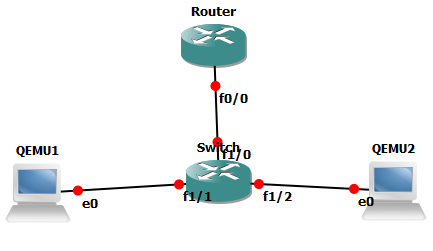
\includegraphics[width=10cm]{fig/topology-vlan.png}
  \caption{Моделируемая топология}
  \label{fig:topology-vlan}
\end{figure}
Допустим, что нам необходимо настроить устройство под маркером \verb`switch` в качестве коммутатора, а устройство
\verb`router` в качестве маршрутизатора. При этом компьютеры \verb`qemu1` и \verb`qemu2` должны быть подключены
к access портам, относящимся к двум разным VLAN'ам, а связь между двумя сетевыми устройствами настроена как \verb`trunk`.

В качестве сетевого оборудования будем использовать Cisco 2691 с подключенным сетевым модулем NM-16NSW.
Для VLANов будут назначены сети 192.168.1.0/24 и 192.168.2.0/24 со статическими адресами соответственно, в качестве
протокола будет использован .1Q. 

\subsection{Подготовка образов}

Перед началом работы, необходимо загрузить образа операционных систем в Glance. В отличии от остальных операций, это действие
является административным, пользователи системы как правило не должны в нем нуждаться. 

В качестве образа Cisco IOS будем 
использовать \verb`c2691-entservicesk9-mz.124-13b.bin`, в качестве образа для виртуальных машин -- ttylinux 16.0.

Для загрузки образов служит команда glance. При загрузке образов Cisco мы должны указать значения свойств 
\verb`hypervisor_type` и \verb`dynamips_platform`. Для образа ttylinux требуется указать лишь значение свойства
\verb`hypervisor_type`:
\begin{lstlisting}
$ glance image-create --name c2691-entservicesk9-mz.124-13b --disk-format raw --container-format bare --is-public True --property hypervisor_type=dynamips --property dynamips_platform=2691 < /path/to/c2691-entservicesk9-mz.124-13b
+------------------------------+--------------------------------------+
| Property                     | Value                                |
+------------------------------+--------------------------------------+
| Property 'dynamips_platform' | c2691                                 |
| Property 'hypervisor_type'   | dynamips                             |
| checksum                     | c03ea442cd0306149821ec58b9aa667d     |
| container_format             | bare                                 |
| created_at                   | 2013-05-19T18:29:06.000862           |
| deleted                      | False                                |
| deleted_at                   | None                                 |
| disk_format                  | raw                                  |
| id                           | 3d778050-6a7a-4380-af96-541e4984ad26 |
| is_public                    | True                                 |
| min_disk                     | 0                                    |
| min_ram                      | 0                                    |
| name                         | c2691-entservicesk9-mz.124-13b       |
| owner                        | None                                 |
| protected                    | False                                |
| size                         | 34347932                             |
| status                       | active                               |
| updated_at                   | 2013-05-19T18:29:06.560694           |
+------------------------------+--------------------------------------+
$ glance image-create --name ttylinux-16.0 --property hypervisor_type=qemu --disk-format iso --container-format bare --is-public True < /path/to/ttylinux.iso
+----------------------------+--------------------------------------+
| Property                   | Value                                |
+----------------------------+--------------------------------------+
| Property 'hypervisor_type' | qemu                                 |
| checksum                   | 38bfe1712504c69c92704391e4ed2d97     |
| container_format           | bare                                 |
| created_at                 | 2013-05-19T18:25:16.239083           |
| deleted                    | False                                |
| deleted_at                 | None                                 |
| disk_format                | iso                                  |
| id                         | dcccddeb-8f39-4ec9-bac9-6401bfcdeeab |
| is_public                  | True                                 |
| min_disk                   | 0                                    |
| min_ram                    | 0                                    |
| name                       | ttylinux-16.0                        |
| owner                      | None                                 |
| protected                  | False                                |
| size                       | 75675648                             |
| status                     | active                               |
| updated_at                 | 2013-05-19T18:25:18.849525           |
+----------------------------+--------------------------------------+
\end{lstlisting}

OpenStack по-умолчанию предоставляет флейворы только для обычных виртуальных машин.
Для того, чтобы устройство c2691 стало доступно в списке допустимых типов узлов, 
так же необходимо создать флейвор при помощи команды \verb`nova-manage`:
\begin{lstlisting}
$ nova-manage flavor create --name c1.2691 --memory 128 --cpu 1 --root_gb=0 --ephemeral_gb=0 --flavor 10 --swap 0 --rxtx_factor 1
\end{lstlisting}
Выделим для этого типа устройств 128 Мб оперативной памяти, а не используемые 
параметры максимального размера дисков выставим в 0. После этого два типа узлов 
являются полностью сконфигурированными, система готова к использованию.

\subsection{Описание топологии в машинном формате}

Очевидно, что моделируемая топология, изображенная на рисунке~\ref{fig:topology-vlan}, состоит из четырех
узлов и трех связей. Таким образом, описание топологии будет содержать четыре элемента в списке \verb`devices` 
и три элемента в списке \verb`wires`:
\lstinputlisting{code/vlan-example.json}
Так же мы указали модель подключенной сетевой карты для коммутатора, а так же идентификаторы образов,
загруженных на предыдущем шаге.

\subsection{Запуск и взаимодействие с виртуальными машинами}

Пользуясь утилитой \verb`curl` для отправки HTTP-запросов, запустим нашу топологию на выполнение:
\begin{lstlisting}
$ curl localhost:5000/mytenant/instances -v -H Content-Type:application/json -d "`cat vlan-example.json`"
{"wires": [{"right": {"device": "Switch", "slot": 0, "port": 0}, "id": "Router_0_0-Switch_1_0", "left": {"device": "Router", "slot": 0, "port": 0}}, {"right": {"device": "Switch", "slot": 1, "port": 1}, "id": "Qemu1_0_0-Switch_1_1", "left": {"device": "Qemu1", "slot": 0, "port": 0}}, {"right": {"device": "Switch", "slot": 1, "port": 2}, "id": "Qemu2_0_0-Switch_1_2", "left": {"device": "Qemu2", "slot": 0, "port": 0}}], "tenant": "mytenant", "devices": [{"name": "Router", "hardware": "c1.2691", "slots": [{"model": "GT96100-FE", "editable": false, "parameters": {}}, {"model": null, "editable": true, "parameters": {}}], "software": "3d778050-6a7a-4380-af96-541e4984ad26", "id": "Router", "metadata": {}}, {"name": "Switch", "hardware": "c1.2691", "slots": [{"model": "GT96100-FE", "editable": false, "parameters": {}}, {"model": "NM-16ESW", "editable": true, "parameters": {}}], "software": "3d778050-6a7a-4380-af96-541e4984ad26", "id": "Switch", "metadata": {}}, {"name": "Qemu1", "hardware": "m1.small", "slots": [{"model": "e1000", "editable": true, "parameters": {}}], "software": "dcccddeb-8f39-4ec9-bac9-6401bfcdeeab", "id": "Qemu1", "metadata": {}}, {"name": "Qemu2", "hardware": "m1.small", "slots": [{"model": "e1000", "editable": true, "parameters": {}}], "software": "dcccddeb-8f39-4ec9-bac9-6401bfcdeeab", "id": "Qemu2", "metadata": {}}], "id": "5199b59c18ab0f3409c26c3c"}
\end{lstlisting}
Ответ будет содержать тело запущенной топологии с идентификатором экземпляра. Получив идентификатор экземпляра, мы можем 
получить веб-консоль для устройств. К примеру, для того, чтобы настроить маршрутизатор, необходимо открыть ссылку
вида \verb`http://localhost:5000/mytenant/instances/5199b59c18ab0f3409c26c3c/webconsole/Router`.

Открывшаяся страница представляет собой стандартный интерфейс консоли ajaxterm, взаимодействие с которым ничем не отличается
от взаимодействия с обычными терминальными клиентами. На рисунке~\ref{fig:example-router-setup} изображен снимок экрана
процесса ввода конфигурации после заполнения базы данных VLAN и настройки транкового порта.
\begin{figure}
  \centering
  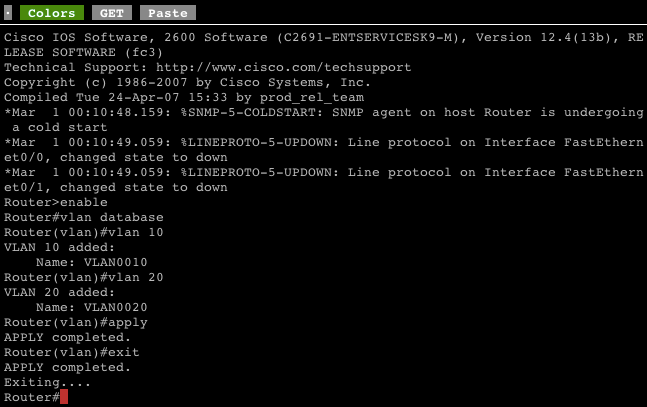
\includegraphics[width=14cm]{fig/example-router-setup-1.png}
  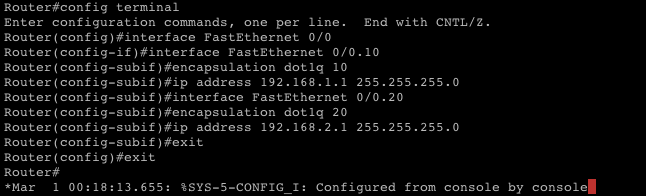
\includegraphics[width=14cm]{fig/example-router-setup-2.png}
  \caption{Настройка маршрутизатора}
  \label{fig:example-router-setup}
\end{figure}

Точно так же мы можем сконфигурировать и коммутатор (рисунок\ref{fig:example-switch-setup}).
\begin{figure}
  \centering
  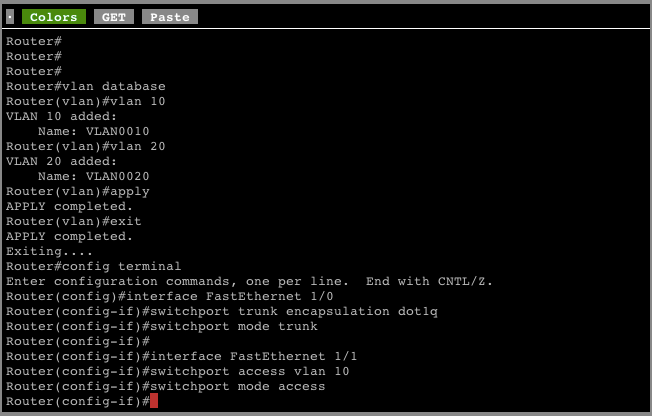
\includegraphics[width=14cm]{fig/example-switch-setup-1.png}
  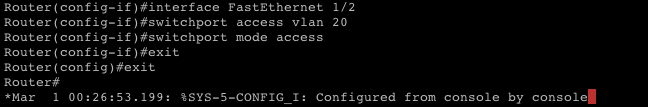
\includegraphics[width=14cm]{fig/example-switch-setup-2.png}
  \caption{Настройка коммутатора}
  \label{fig:example-switch-setup}
\end{figure}

Работа с PC-совместимыми виртуальными машинами ничем не отличается от работы с сетевым оборудованием, для этого
используется все тот же терминал ajaxterm. На рисунке~\ref{fig:example-pc-setup} показан процесс настройки и проверки работы
статических адресов. В конце концов, осталось только окончательно проверить правильность маршрутизации при помощи команды 
traceroute, как это продемонстрировано на рисунке~\ref{fig:example-pc-traceroute}.

\begin{figure}
  \centering
  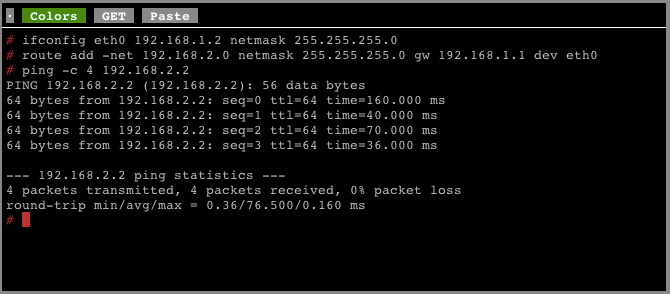
\includegraphics[width=14cm]{fig/example-pc-setup-1.png}
  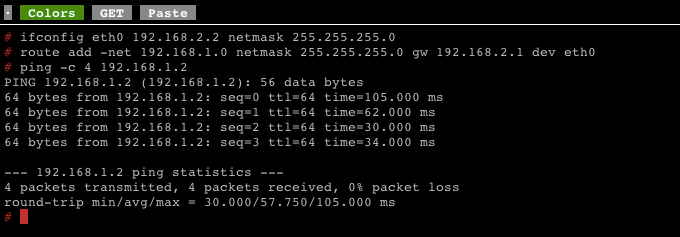
\includegraphics[width=14cm]{fig/example-pc-setup-2.png}
  \caption{Настройка виртуальных машин}
  \label{fig:example-pc-setup}
\end{figure}

\begin{figure}
  \centering
  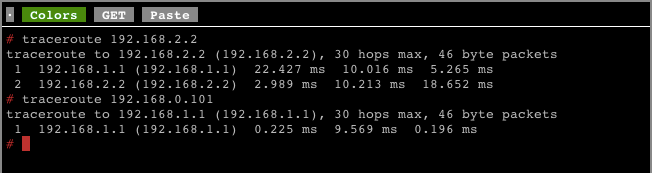
\includegraphics[width=14cm]{fig/example-pc-traceroute.png}
  \caption{Проверка правильности работы маршрутизации}
  \label{fig:example-pc-traceroute}
\end{figure}



